{ % all template changes are local to this group.
    \setbeamertemplate{navigation symbols}{}
    \begin{frame}<article:0>[plain,noframenumbering]
        \begin{tikzpicture}[remember picture,overlay]
            \node[at=(current page.center)] {
                
\includegraphics[keepaspectratio,
                                 width=0.75\paperwidth,
                                 height=\paperheight]{LeeLogo}
            };
        \end{tikzpicture}
     \end{frame}
}

\setchessboard{
smallboard,
showmover=false,
color=red
}

\begin{frame}[fragile]{Ablauf und Ziele von heute}
\begin{itemize}[<+->]
    \item Was bisher geschah? (previously im EF-Informatik)
    \item Herleitung und Diskussion der berühmten Fibonacci-Folge
    \item Umsetzung rekursiver Programme in Computern
    \item diverse Anwendungen
\end{itemize}
\end{frame}

\begin{frame}[fragile]{rekursive Berechnung von $5!$}
\begin{align*}
    \textcolor{Red}{5!} &= 5\cdot\underbrace{4\cdot 3\cdot 2\cdot 1}_{\textcolor{Blue}{4!}} \\
    \textcolor{Blue}{4!} &= 4\cdot\underbrace{3\cdot 2\cdot 1}_{\textcolor{Green}{3!}} \\
    \textcolor{Green}{3!} &= 3\cdot\underbrace{2\cdot 1}_{\textcolor{Goldenrod}{2!}} \\
    \textcolor{Goldenrod}{2!} &= 2\cdot\underbrace{1}_{\textcolor{Fuchsia}{1!}} \\
    \textcolor{Orchid}{1!} &= 1\cdot\underbrace{0!}_{1} = 1
\end{align*}
\end{frame}

\begin{frame}[fragile]{rekursive Berechnung von $5!$}
Durch \textit{Rückwertseinsetzen} erhalten wir nun den Wert für $5!$:
\begin{align*}
    \textcolor{Orchid}{1!} &= 1\cdot 0! = 1 \\
    \textcolor{Goldenrod}{2!} &= 2\cdot\textcolor{Orchid}{1!} = 2\cdot 1 = 2 \\
    \textcolor{Green}{3!} &= 3\cdot \textcolor{Goldenrod}{2!} = 3\cdot 2 = 6 \\
    \textcolor{Blue}{4!} &= 4\cdot\textcolor{Green}{3!} = 4\cdot 6 = 24 \\
    \textcolor{Red}{5!} &= 5\cdot\textcolor{Blue}{4!} = 5\cdot 24 = 120.
\end{align*}
\end{frame}

\begin{frame}[fragile]{rekursive Definition von $n!$}
Es sei $n$ eine natürliche Zahl. Dann definieren wir die Fakultät $n!$ von $n$ durch
\[
  n! := 
  \begin{cases}
    1, &\text{falls $n=0$, (Rekursionsanfang)} \\
    n(n-1)!, & \text{falls  $n\geq 1$. (Rekursionsschritt)}
  \end{cases}
\]
\end{frame}

\begin{frame}[fragile]{rekursive Berechnung von $n!$}
\begin{lstlisting}[language=Python]
def factorial(n):
    if n == 0:
        return 1
    else:
        return n * factorial(n-1)
\end{lstlisting}
\end{frame}

\begin{frame}[fragile]{Definition und Berechnung der Potenz $a^n$}
Sei $a\in\R$ und $n$ eine natürliche Zahl. Wir definieren den Potenzausdruck $a^n$ rekursiv durch
\[
  a^n := 
  \begin{cases}
    1, &\text{falls $n=0$, (Rekursionsanfang)} \\
    a\cdot a^{n-1}, & \text{falls  $n\geq 1$. (Rekursionsschritt)}
  \end{cases}
\]
\end{frame}

\begin{frame}[fragile]{Definition und Berechnung der Potenz $a^n$}
\begin{lstlisting}[language=Python]
def potenz(a,n):
    if n == 0:
        return 1
    else:
        return a * potenz(a,n-1)
\end{lstlisting}
\end{frame}

\begin{frame}[fragile]{Definition und Berechnung der Potenz $a^n$}
\begin{lstlisting}[language=Python]
def potenz(a,n):
    if n == 0:
        return 1
    else:
        return a * potenz(a,n-1)
\end{lstlisting}
\end{frame}


\begin{frame}[fragile]{Summe aller Listeneinträge}
In Python ist eine Liste \pythoninline{L} von reellen Zahlen gegeben. Schreiben Sie eine Python-Funktion \pythoninline{sum_rek(L)}, welche rekursiv die Summe der Zahlen in der Liste berechnet. Es kann angenommen werden, dass die Länge der Liste $\geq 1$ ist.
\begin{lstlisting}[language=Python]
def sum_rek(L):
    if len(L) == 1:
        return L[0]
    else:
        return sum_rek(L[:-1]) + L[-1]
\end{lstlisting}
Dabei ist \pythoninline{L[-1]} das hinterste Element der Liste und \pythoninline{L[:-1]} die gesamte Liste ohne das hinterste Element.
\end{frame}



\begin{frame}[fragile]{Palindrome}
Ein Wort heisst \textit{Palindrom}, falls das Wort vorwärts und rückwärts genau gleich gelesen wird.\\
Beispiele:
\begin{itemize}
    \item neben
    \item Rentner
    \item Otto
    \item Lagerregal
\end{itemize}
Das \textit{leere Wort}, also das Wort der Länge $0$, ist ebenfalls ein Palindrom. Schreiben Sie ein rekursives Python-Programm, welches entscheidet, ob ein gegebenes Wort \verb|w| ein Palindrom ist oder nicht.
\end{frame}


\begin{frame}[fragile]{Palindrome}
\begin{lstlisting}[language=Python]
def check_palindrom(w):
    w = w.upper()
    if len(wort) <= 1:
        return True
    elif w[0] != w[-1]:
        return False
    return check_palindrom(w[1:-1])
\end{lstlisting}
\end{frame}

\begin{frame}[fragile]{Palindrome}
Lösung von Schafer, Gondorf et al., 2023
\lstset{basicstyle=\ttfamily\scriptsize}
\begin{lstlisting}[language=Python]
def check_palindrom(w):
    return (True if len(w) <= 1 else (check_palindrom(w[1:-1]) if w[0].lower() == w[-1].lower() else False))
\end{lstlisting}
\lstset{basicstyle=\ttfamily\normalsize}
\end{frame}

\begin{frame}[fragile]{Fibonacci-Folge}
In der zweiten Fassung des Buches \textit{Liber abbaci} (Buch der Rechenkunst) beschrieb der italienische Mathematiker \textit{Leonardo da Pisa}, bekannt als \textit{Fibonacci}, das Wachstum einer Kaninchenpopulation. Dies war im Jahre 1202.
\end{frame}


\begin{frame}[fragile]{Fibonacci-Folge}
\begin{itemize}[<+->]
    \item Jedes geschlechtsreife Paar Kaninchen wirft pro Monat genau ein neues Paar Kaninchen (ein Weibchen und ein Männchen). Die Austragungszeit (Dauer der Schwangerschaft) dauert bei Kaninchen also immer genau einen Monat. Jeden Monat kommt also eine neue Generation von Kaninchen zur Welt.
    \item Ein neugeborenes Paar von Kaninchen wird erst am Ende seines ersten Lebensmonats geschlechtsreif und wirft entsprechend erst Ende seines zweiten Lebensmonats sein erstes Paar Kaninchen.
    \item Kein Kaninchen stirbt, verlässt das betrachtete System oder wird, ausser durch Geburt, in das System hineingebracht.
\end{itemize}
\end{frame}


\begin{frame}[fragile]{Fibonacci-Folge}
\begin{itemize}[<+->]
    \item Sei $G_n$ die Anzahl der geschlechtsreifen Kaninchenpaare und $g_n$ die Anzahl der nicht geschlechtsreifen Kaninchenpaare der Generation $n$ für $n\in\N$.
    \item Beachten Sie, dass die gesamte Anzahl der Kaninchenpaare der Generation $n$ damit der Summe $F_n := G_n+g_n$ entspricht.
\end{itemize}
\end{frame}


\begin{frame}[fragile]{Fibonacci-Folge}
Sei $n\in\N$.
\begin{itemize}[<+->]
\item Es gilt
\begin{align*}
    G_{n+2} = G_{n+1} + g_{n+1},
\end{align*}
da die geschlechtsreifen Kaninchen $G_{n+1}$ der Generation $n+1$ auch einen Monat später noch geschlechtsreif sein werden und die nicht geschlechtsreifen Kaninchen $g_{n+1}$ der Generation $n+1$ einen Monat später geschlechtsreif sein werden.
\item Völlig analog begründet man die Gleichung
\begin{align*}
    G_{n+1} = G_{n} + g_{n}.
\end{align*}
\item Offensichtlich gilt zudem
\begin{align*}
    g_{n+2}  = G_{n+1}.
\end{align*}
\end{itemize}
\end{frame}

\begin{frame}[fragile]{Fibonacci-Folge}
Wir haben also drei Gleichungen für die Population:
\begin{align}\label{eq:Fib1}
    \textcolor{Blue}{G_{n+2}} = \textcolor{Red}{G_{n+1}} +  \textcolor{Blue}{g_{n+1}}
\end{align}
\begin{align}\label{eq:Fib2}
    \textcolor{Red}{G_{n+1}} = \textcolor{Red}{G_{n}} + \textcolor{Red}{g_{n}}
\end{align}
\begin{align}\label{eq:Fib3}
    \textcolor{Purple}{g_{n+2}}  = \textcolor{Purple}{G_{n+1}}
\end{align}
Wir setzen nun Gleichung \ref{eq:Fib2} in Gleichung \ref{eq:Fib1} ein und erhalten:
\begin{align*}
    \textcolor{Blue}{G_{n+2}} &= \textcolor{Red}{G_{n}} + \textcolor{Red}{g_{n}} + \textcolor{Blue}{g_{n+1}} \\
    &\iff \\
    \underbrace{\textcolor{Blue}{G_{n+2}} + \textcolor{Purple}{g_{n+2}}}_{F_{n+2}} &= \underbrace{\textcolor{Purple}{G_{n+1}} + \textcolor{Blue}{g_{n+1}}}_{F_{n+1}} + \underbrace{\textcolor{Red}{G_{n}} + \textcolor{Red}{g_{n}}}_{F_n}.
\end{align*}
\end{frame}

\begin{frame}[fragile]{Fibonacci-Folge}
Für die Gesamtzahl der Population der Kaninchenpaare gilt also
\begin{align*}
    F_{n+2} = F_{n+1} + F_{n}
\end{align*}
für alle $n\in\N$. Für Generation $n=0$ definieren wir $G_0:=0$ und $g_0:=0$. Zu Beginn, also in der Generation $n=1$, wird ein erstes Paar von Kaninchen in das System eingeführt. Dieses erste Paar wird erst nach einem Monat geschlechtsreif. Es gilt also $G_1=0$ und $g_1=1$. Somit besteht die Generation $n=2$ immer noch aus nur einem Paar Kaninchen: $G_2=1$ und $g_2=0$. Die Generation $n=3$ aus zwei Paaren: $G_3=1$ und $g_3=1$. Logisch fortgeführt findet man die sogenannte \textit{Fibonacci-Folge}.
\begin{align*}
    &F_0 = 0, F_1 = 1, F_2 = 1, F_3 = 2, F_4 = 3, F_5 = 5, F_6 = 8,\\
    &F_7 = 13, F_8 = 21, F_9 = 34, F_{10} = 55, F_{11} = 89, \ldots
\end{align*}
\end{frame}

\begin{frame}[fragile]{Fibonacci-Folge}
Die Fibonacci-Folge ist somit rekursiv definiert durch
\[
  F_n := 
  \begin{cases}
    0, &\text{falls $n=0$, (Rekursionsanfang)} \\
    1, &\text{falls $n=1$, (Rekursionsanfang)} \\
    F_{n-1} + F_{n-2}, & \text{falls  $n\geq 2$. (Rekursionsschritt)}
  \end{cases}
\]
\end{frame}

\begin{frame}[fragile]{Spirale}
\begin{figure}
    \centering
    \includesvg[scale=0.4]{Goldene_Spirale}
\end{figure}
\end{frame}

\begin{frame}[fragile]
\begin{figure}
    \centering
    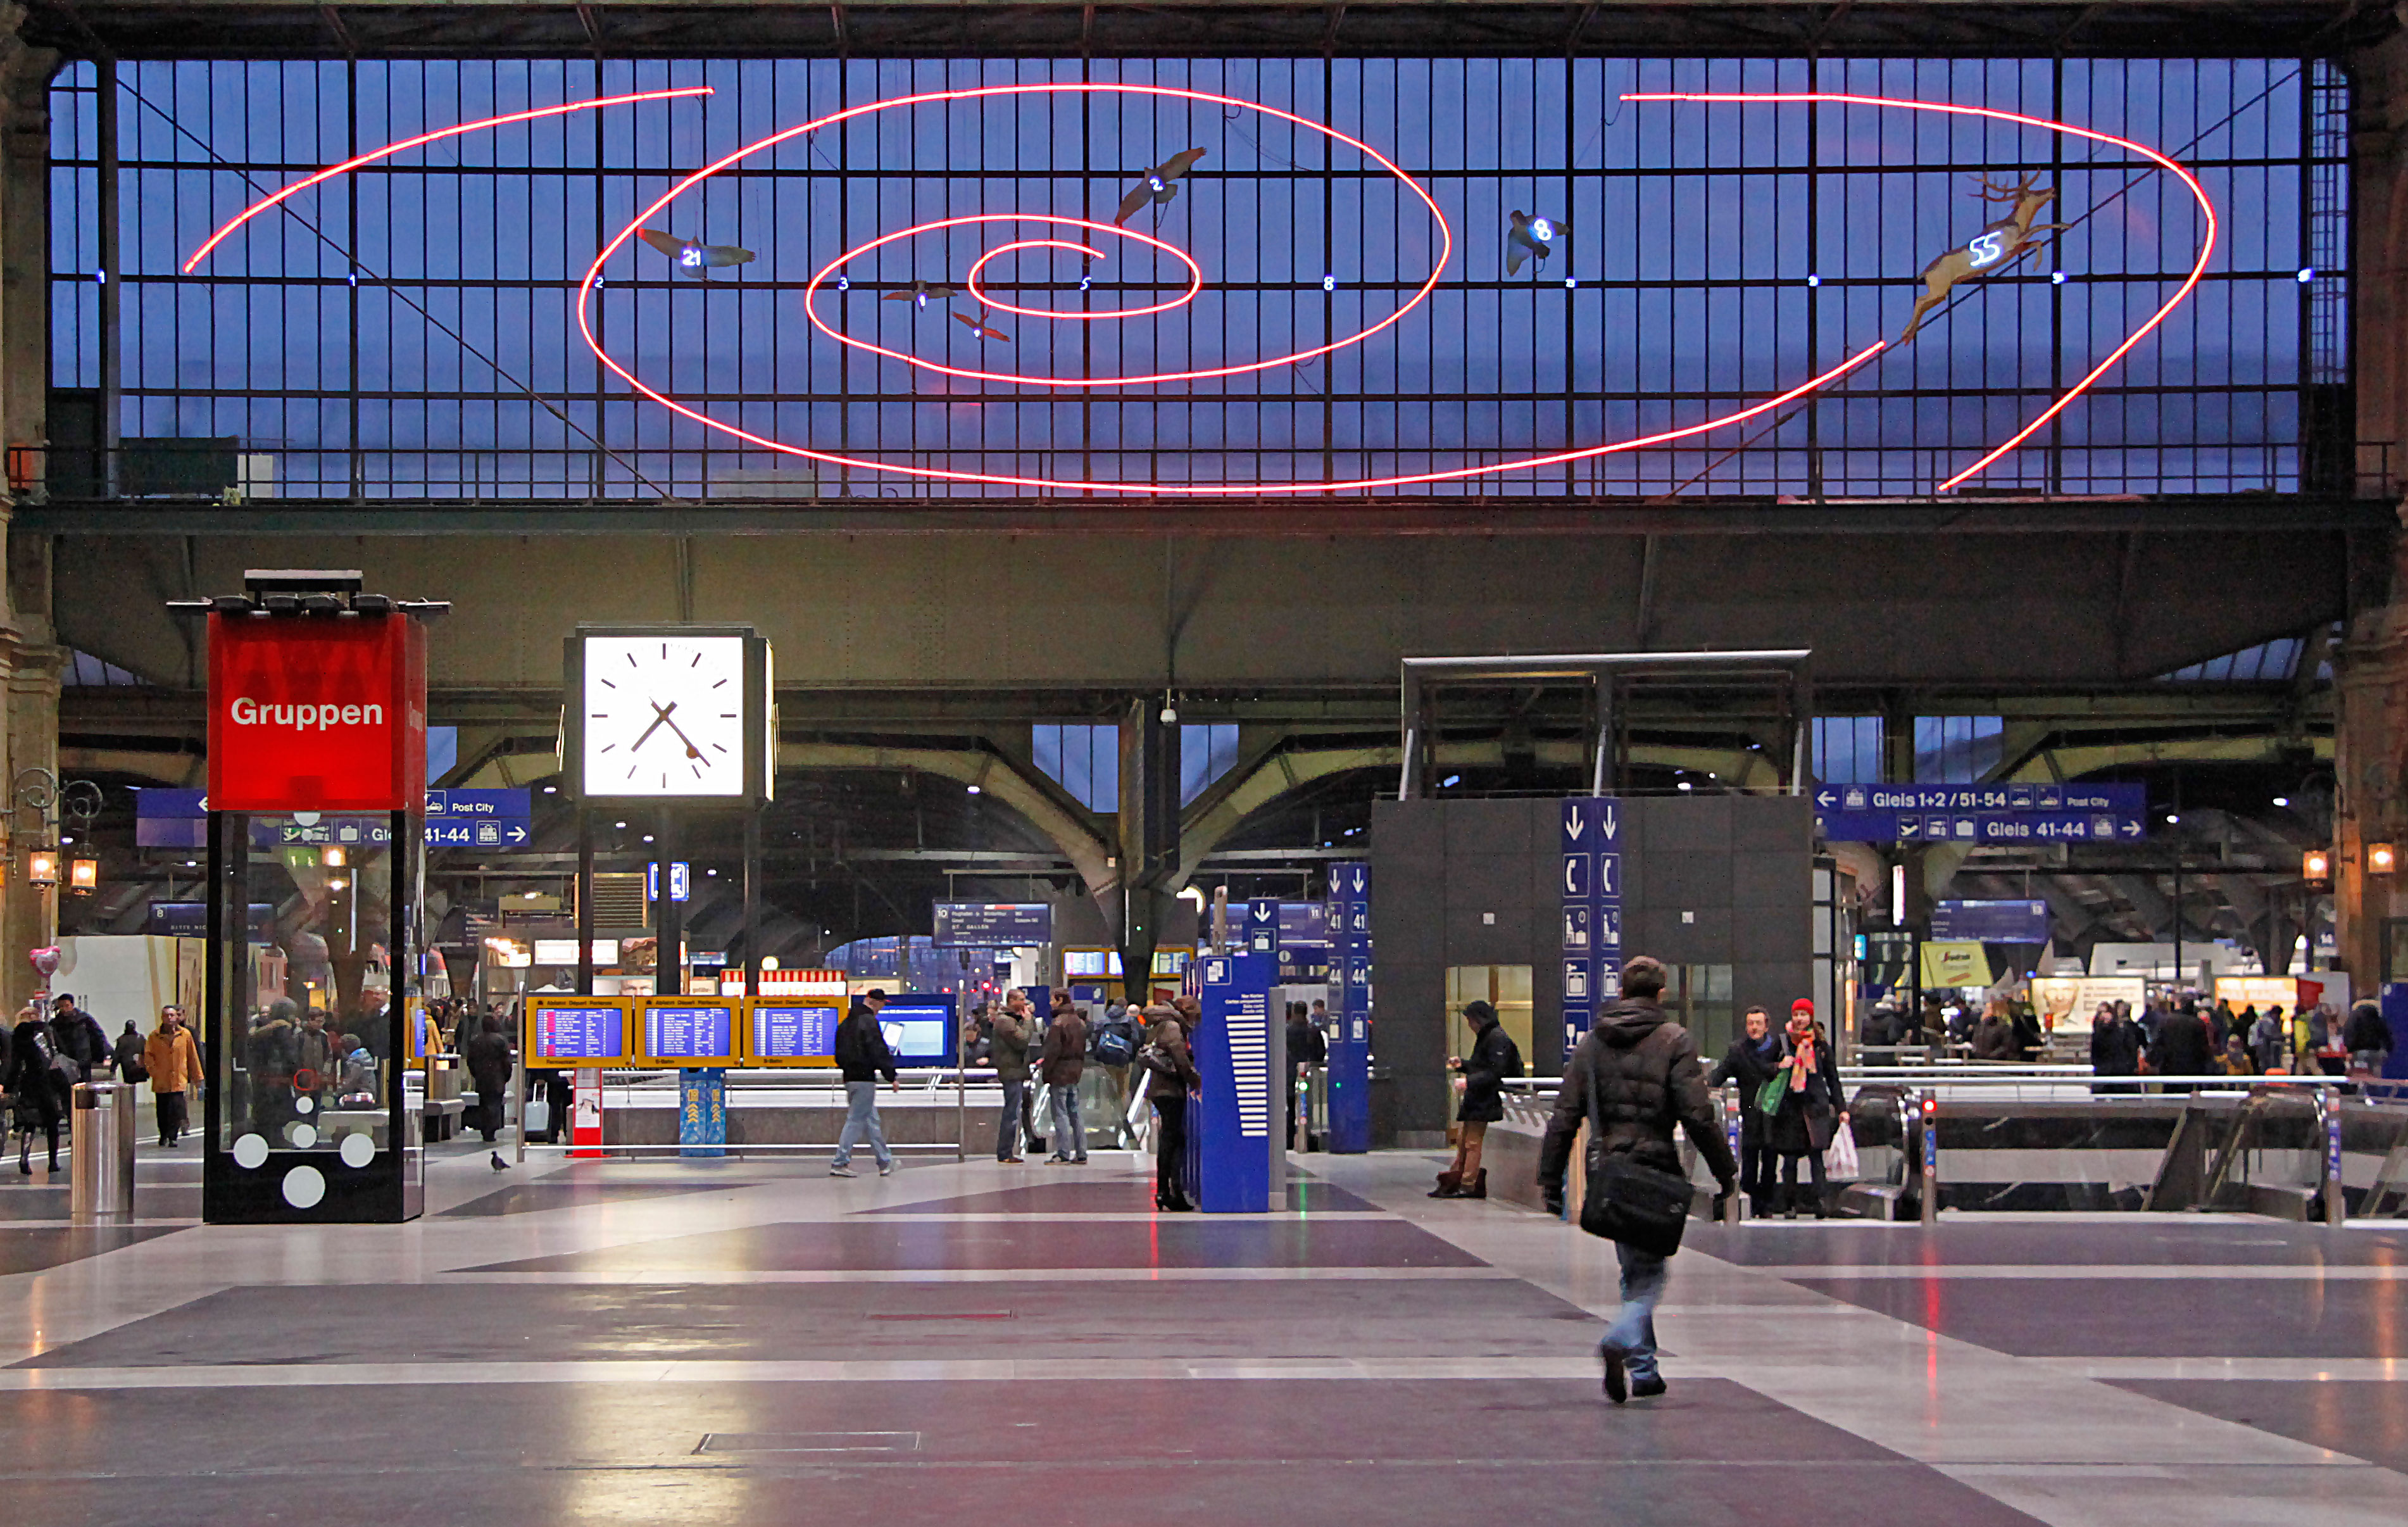
\includegraphics[width=1\textwidth]{Fibonacci_numbers_in_Zurich_HB.jpg}
\end{figure}
\end{frame}

\begin{frame}[fragile]{Aufgaben}
\begin{itemize}
    \item Aufgabe 3.11 (A3.7)
    \item Aufgabe 3.12 (A3.8) $\leftarrow$ die Schnellen können hier die Zeit nutzen, um einen eindrücklichen Plot zu erstellen.
\end{itemize}
\end{frame}

\begin{frame}[fragile]{Fibonacci-Folge auf einem 8-Bit Computer :)}
\end{frame}

\begin{frame}[fragile]{Technische Umsetzung rekursiver Programme}
\begin{lstlisting}[language=Python]
def binaryStrings(n, w = ''):
    if n == 0:
        print(w)
        return
    binaryStrings(n-1, w + '0')
    binaryStrings(n-1, w + '1')
    #return # optional
\end{lstlisting}
\end{frame}

\begin{frame}[fragile]{Binäre Strings ohne aufeinanderfolgende Einsen}
Bearbeiten Sie Kapitel 4 (Binäre Strings ohne
aufeinanderfolgende Einsen).
\end{frame}